\newpage 

\subsection{Task, Data, and Pipeline Parallelism}

Task, data, and pipeline parallelism are three common forms of parallelism:

\begin{Def}[Task Parallelism]

    \textbf{Task parallelism} involves running multiple tasks simultaneously. Each task is independent and can run in parallel with other tasks,
    perhaps even on the same data.
\end{Def}
\noindent
In essence, we may think \underline{same data, different tasks}:
\begin{figure}[h]
    \centering
    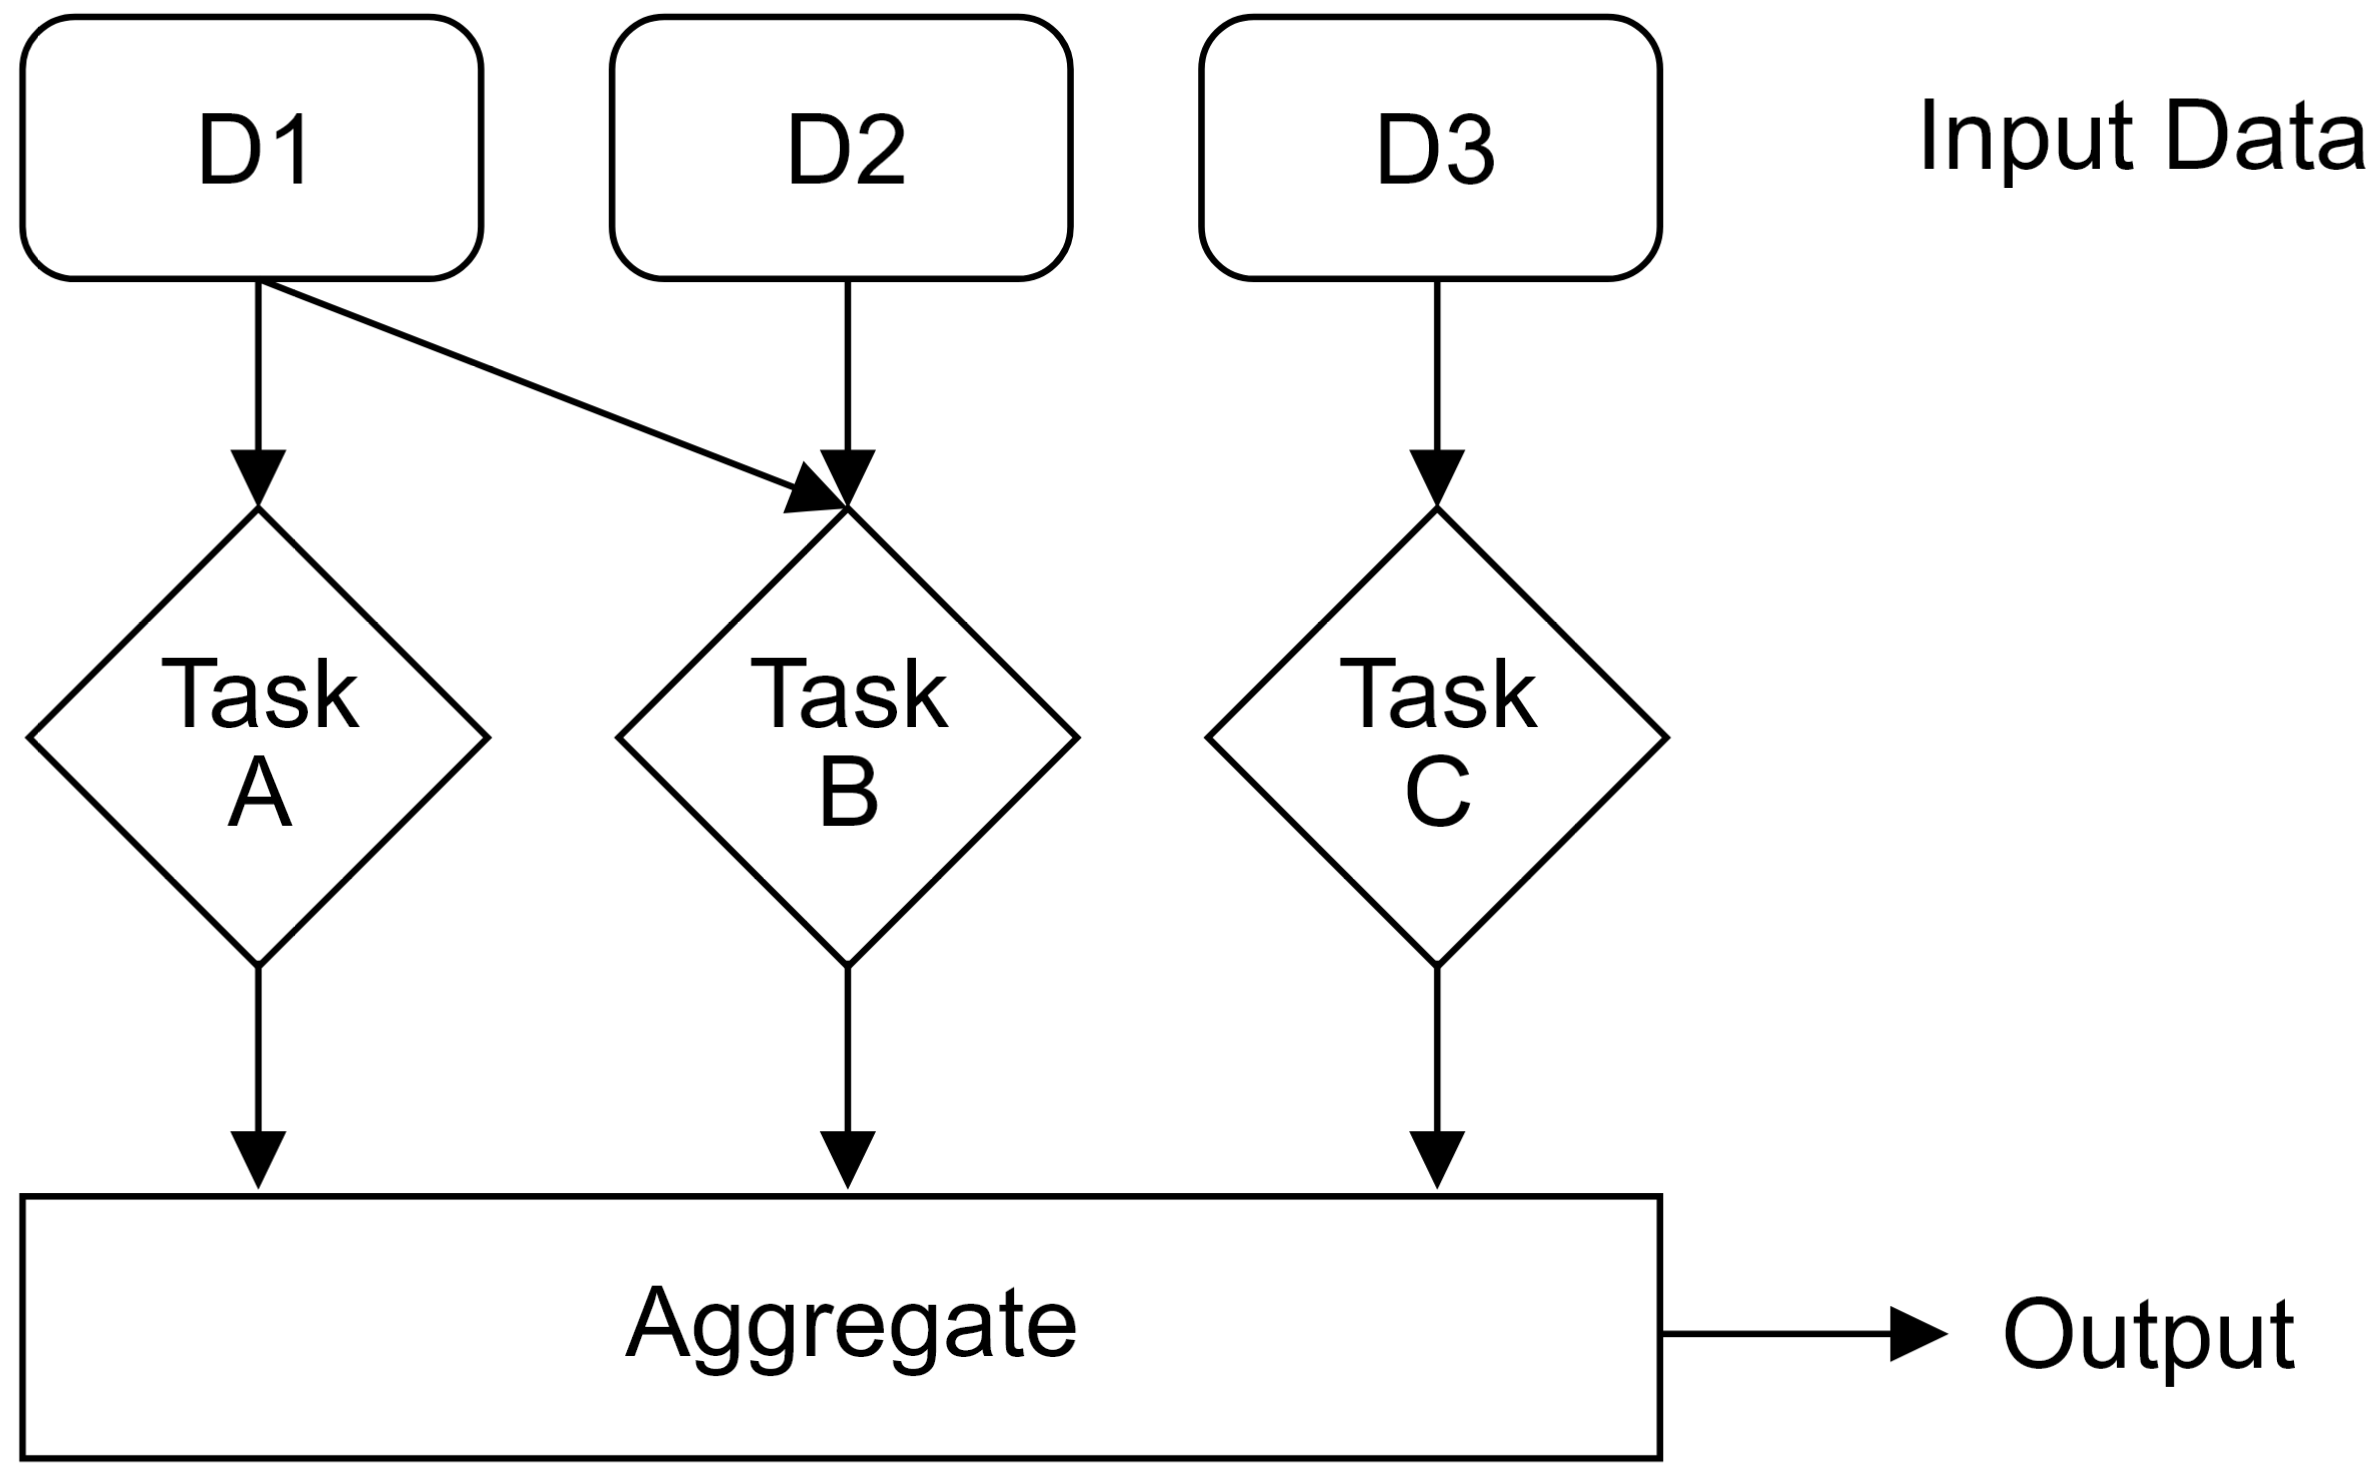
\includegraphics[width=0.5\textwidth]{./Sections/rpc_2/tpar.png}
    \caption{Task Parallelism Culminating into an Aggregate Result}
\end{figure}
\noindent

\vspace{-1em}
\begin{Def}[Data Parallelism]

    \textbf{Data parallelism} involves running the same task on multiple data items. Each task is identical, but the data is different.
\end{Def}
\noindent
We may think \underline{same task, different data}:
\begin{figure}[h]
    \centering
    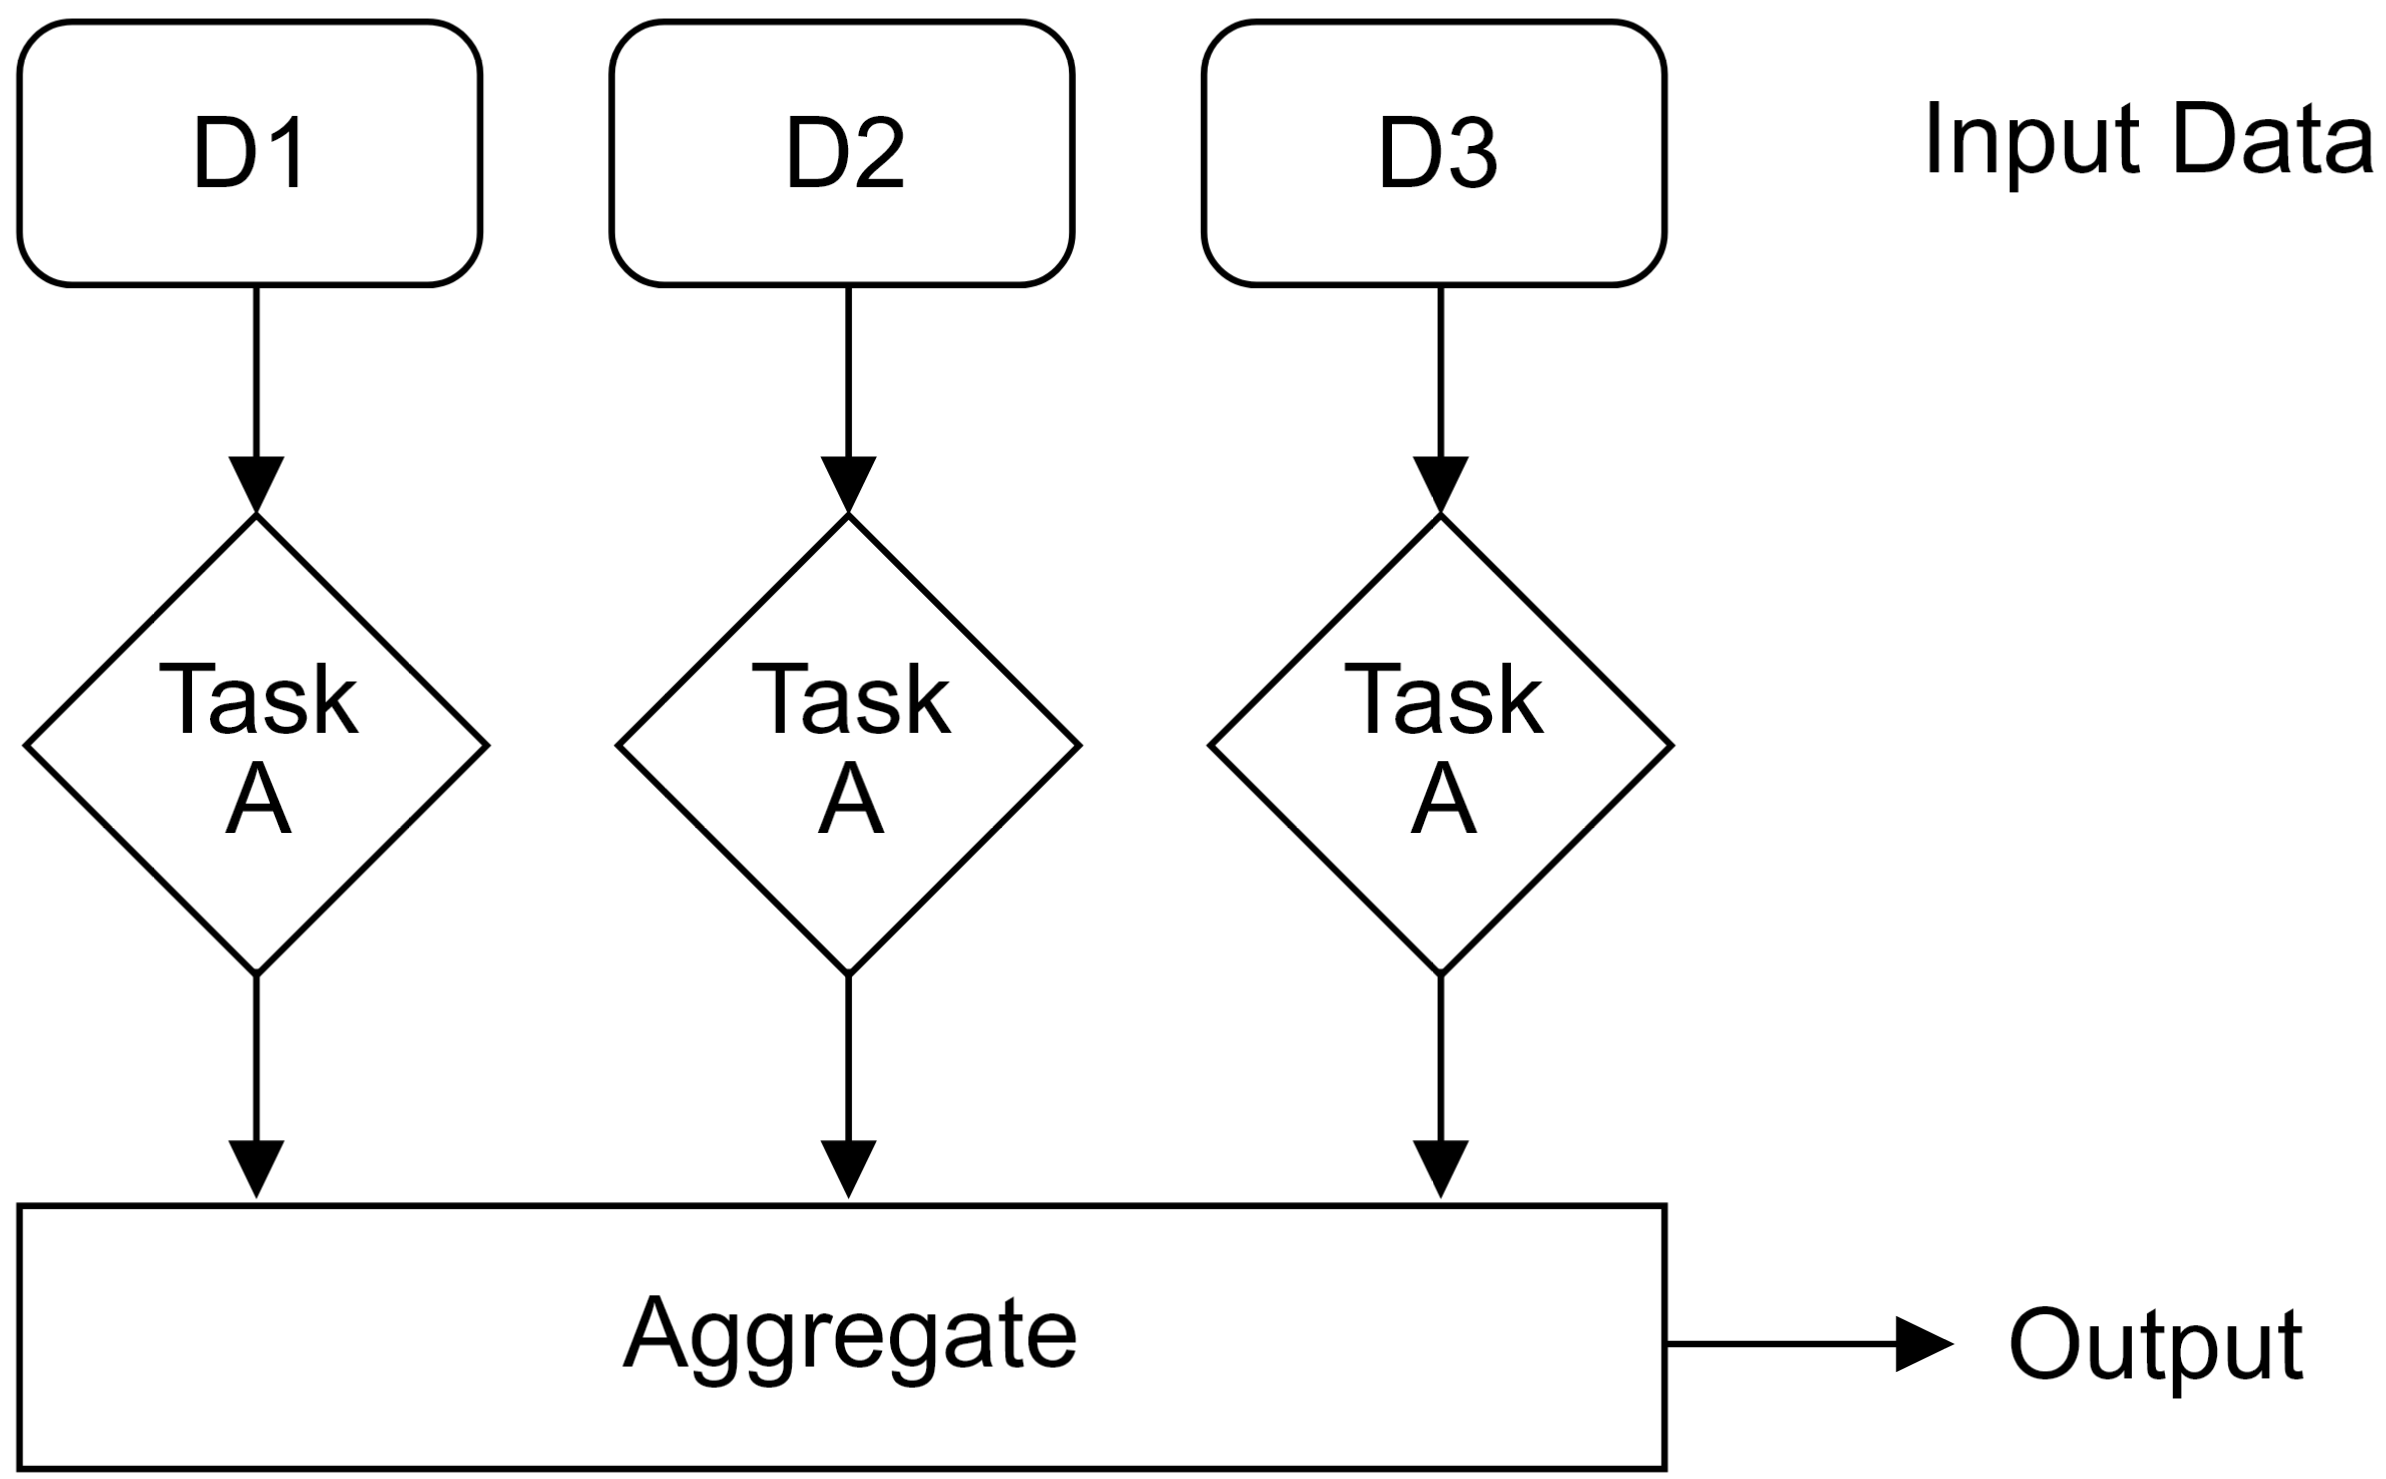
\includegraphics[width=0.5\textwidth]{./Sections/rpc_2/dpar.png}
    \caption{Data Parallelism Culminating into an Aggregate Result}
\end{figure}

\newpage 
\noindent
To continue, we have:
\begin{Def}[Pipeline Parallelism]

    \textbf{Pipeline parallelism} involves breaking a task into multiple stages, each of which can be executed concurrently. The output of one stage is the input to the next stage.
\end{Def}

For instance, consider the following pipeline:
\begin{itemize}
    \item \textbf{Task A}: ``Search for a flight.'' (1 time unit)
    \item \textbf{Task B}: ``Book a flight.'' (1 time unit)
\end{itemize}

\noindent
First consider the scenario where we only have one resource to work with, resulting in concurrency:
\begin{figure}[h]
    \centering
    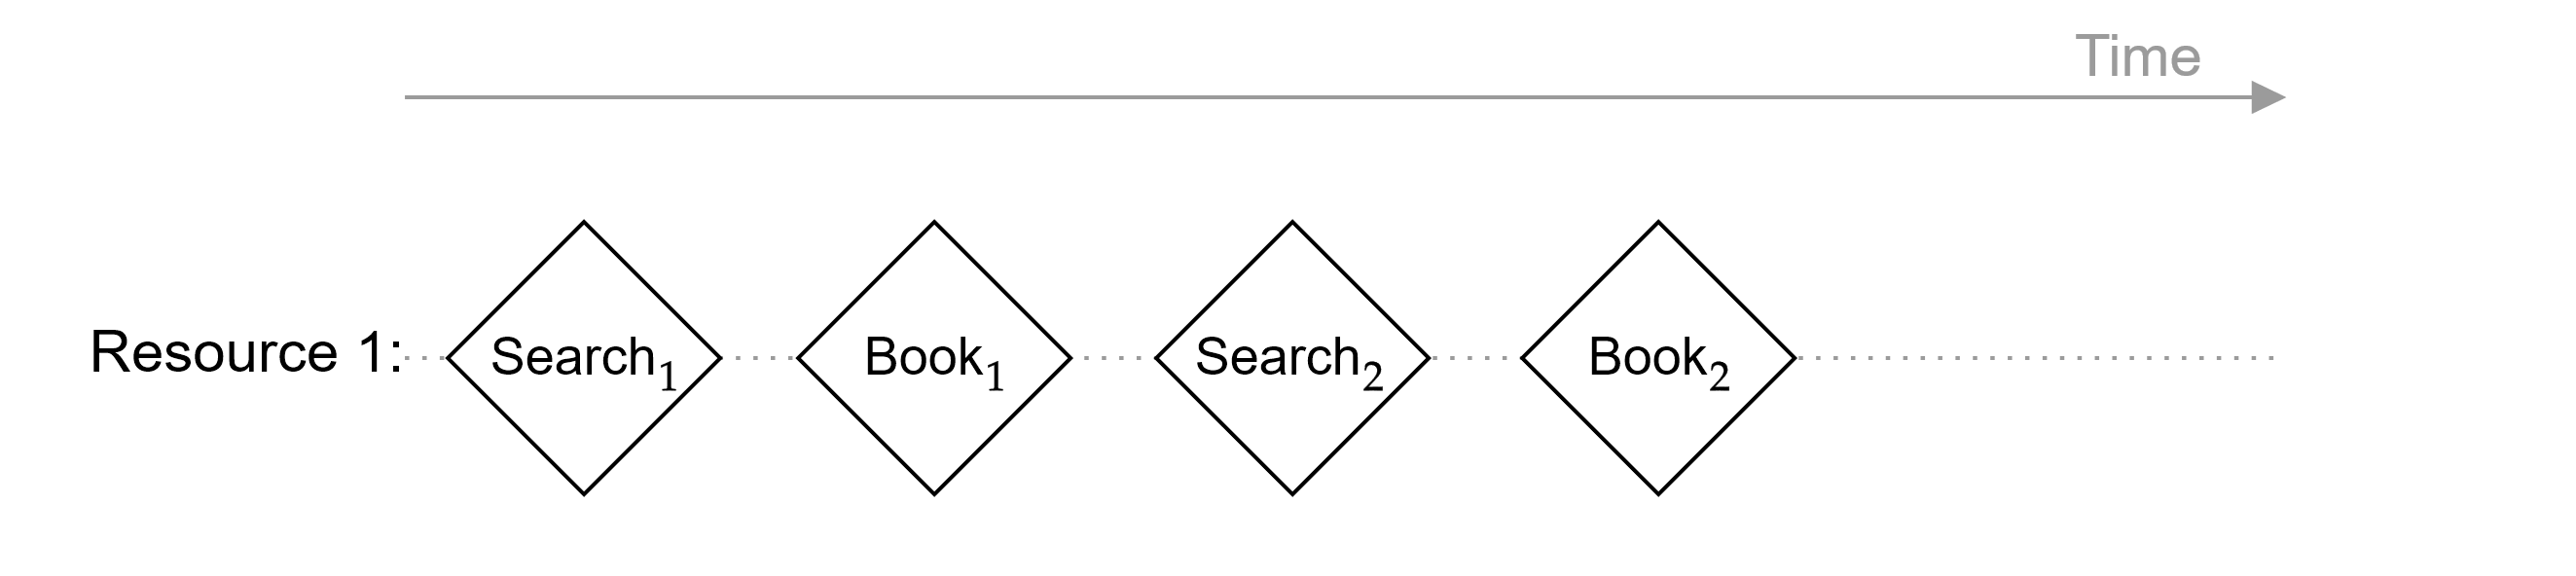
\includegraphics[width=1\textwidth]{./Sections/rpc_2/ppar.png}
    \caption{Searching and Booking flights concurrently}
\end{figure}

\noindent
Now consider the scenario where we have two resources to work with, resulting in parallelism:
\begin{figure}[h]
    \centering
    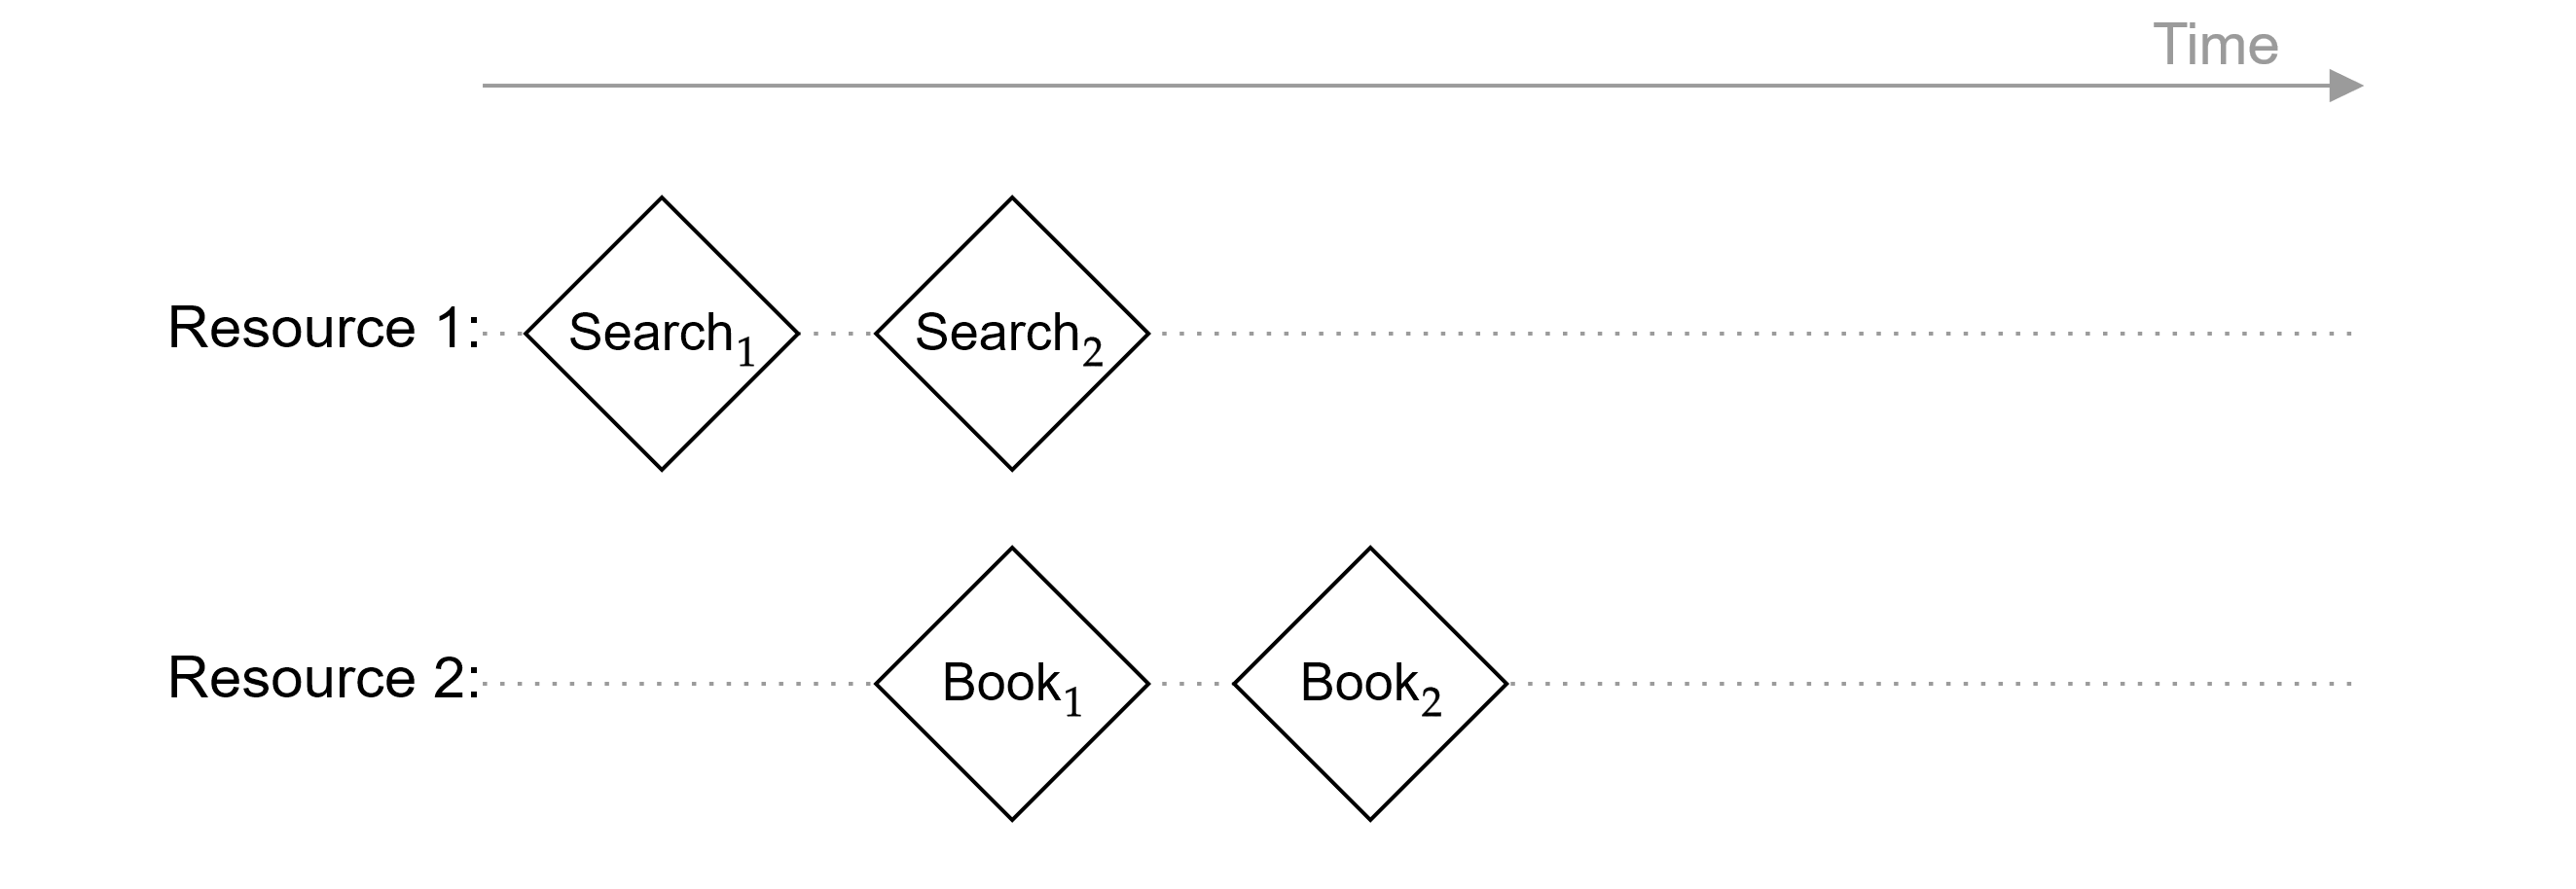
\includegraphics[width=1\textwidth]{./Sections/rpc_2/ppar_2.png}
    \caption{Searching and Booking flights in parallel}
\end{figure}
\noindent
In this case, once the first search is done, we can start booking the flight and search for the next flight in parallel.
\newpage 

\subsection{Arrays \& Slices in Go}

\noindent
Arrays in Go act like arrays in other languages, a fixed-size collection of items of the same type. Slices, on the other hand, allow us to work with a dynamically-sized sequence of elements.

\begin{Def}[Arrays in Go]

    An \textbf{array} in Go is a fixed-size collection of elements of the same data type. Arrays in Go are value types, meaning they are copied when assigned to a new variable.\\
    
    \noindent
    Arrays are declared using the syntax:
    \begin{lstlisting}[language=Go]
    var arr [size]Type
    \end{lstlisting}
    
    \noindent
    For example, an array of integers with 5 elements:
    \begin{lstlisting}[language=Go]
    var numbers [5]int
    \end{lstlisting}
    
    \noindent
    Elements in an array can be accessed using zero-based indexing:
    \begin{lstlisting}[language=Go]
    numbers[0] = 10  // Assign value
    fmt.Println(numbers[0]) // Access value
    \end{lstlisting}
    
    \noindent
    Arrays cannot be resized, and their size must be known at compile time. For dynamic collections, slices are preferred.
\end{Def}

\begin{Example}[Doubling Items in an array]

    Consider the following example where we double each element in an array:
    \begin{lstlisting}[language=Go, numbers=none]
    package main

    import "fmt"

    func main() {
        // Initialize an array
        numbers := [5]int{1, 2, 3, 4, 5}

        // Double each element in the array
        for i := 0; i < len(numbers); i++ {
            numbers[i] *= 2 // Shorthand for numbers[i] = numbers[i] * 2
        }

        // Print the modified array
        fmt.Println(numbers)
    }
    // Output: [2 4 6 8 10]
    \end{lstlisting}
\end{Example}

\newpage
    
\noindent
In contrast, slices:

\begin{Def}[Slices in Go]
    
    A \textbf{slice} is a dynamically-sized reference to a portion of a single underlying array.

    \noindent
    Slices are declared using square brackets without specifying a fixed size:
    \begin{lstlisting}[language=Go]
    var numbers []int // A slice of integers
    \end{lstlisting}
    
    \noindent
    Slices are typically created using the \snippet{make} function or by slicing an existing array:
    \begin{lstlisting}[language=Go]
    // Using make()
    numbers := make([]int, 5) // Creates a slice with length 5
    
    // Slicing an array
    arr := [5]int{1, 2, 3, 4, 5}
    slice := arr[1:4] // Slice from index 1 to 3 -> {2, 3, 4}
    \end{lstlisting}
    
    \noindent
    Slices maintain a reference to the original array, meaning modifications affect both:
    \begin{lstlisting}[language=Go]
    arr := [5]int{1, 2, 3, 4, 5}
    slice := arr[1:3]
    slice[0] = 99 // Modifies arr[1] as well
    fmt.Println(arr)  // Output: [1 99 3 4 5]
    \end{lstlisting}

    \noindent
    The \snippet{append()} function modifies slices given there's enough capacity:
    \begin{lstlisting}[language=Go]
    arr := [5]int{1, 2, 3, 4, 5}
    slice := arr[:1] // Slice from index 0 to 0 -> {1}
    slice = append(slice, 7, 8) // Adds elements to the slice
    fmt.Println(slice) // Output: [1 7 8]
    fmt.Println(arr)   // Output: [1 7 8 4 5] (modified)
    \end{lstlisting}

    \noindent
    If \snippet{append()} exceeds the slice's capacity, a new array is allocated and referenced by the slice:
    \begin{lstlisting}[language=Go]
    ... // Previous code
    fmt.Println(cap(slice)) // Output: 5 (capacity of the slice)
    slice = append(slice, 7, 8, 9, 10, 11) // Exceeds capacity, (6 total)
    fmt.Println(slice) // Output: [1 7 8 9 10 11]
    fmt.Println(arr)   // Output: [1 2 3 4 5] (unchanged)
    \end{lstlisting}

    \noindent
    To copy an array to a slice, use the \snippet{copy()} function:
    \begin{lstlisting}[language=Go]
    arr := [5]int{1, 2, 3, 4, 5}
    slice := make([]int, len(arr))
    copy(slice, arr) // Syntax: copy(destination, source)
    slice[0] = 99
    fmt.Println(slice) // Output: [99 2 3 4 5]
    fmt.Println(arr)   // Output: [1 2 3 4 5] (unchanged)
    \end{lstlisting}
\end{Def}

\newpage 
\subsection{Repeating Tasks: Tick and Ticker in Go}

In Go, the \snippet{time} package provides two types for repeating tasks at regular intervals:

\begin{Def}[\texttt{time.Tick} and \texttt{time.Ticker} in Go]

    The \texttt{time} package in Go provides two mechanisms for scheduling repeated tasks at fixed intervals:
    
    \begin{itemize}
        \item \textbf{\snippet{time.Tick(duration)}}: Returns a channel that sends the current time at regular intervals. It is a convenience function but \textbf{}{cannot be stopped}.
        \item \textbf{\snippet{time.NewTicker(duration)}}: Creates a \snippet{Ticker} object, which provides a \snippet{.Stop()} method to halt the ticker. Additionally the \snippet{.C} returns a channel from which the signal can be read.
        This channel is read only, hence a type of \snippet{<-chan time.Time}.
    \end{itemize}
\end{Def}

\begin{Example}[Record a signal n times every second]

    Say we want to record a signal $n$ times every second. We can use a \snippet{time.Ticker}:
    \begin{lstlisting}[language=Go, numbers=none]
    package main
    import "fmt"; import "time"; import "sync"
    
    func Status(ch <-chan time.Time, wg *sync.WaitGroup) {
        defer wg.Done()
        <-ch // Wait for signal
        fmt.Println("Status: OK")
    }
    
    func main() {
    
        n := 5
        ticker := time.NewTicker(time.Second)
        tickerChan := ticker.C
        var wg sync.WaitGroup
    
        // Spawns n goroutines which waiting for the signal
        for i := 0; i < n; i++ {
            wg.Add(1)
            go Status(tickerChan, &wg)
        }
        wg.Wait()
        ticker.Stop()
    }
    \end{lstlisting}

    \noindent
    This type of example can be extended to perform any task at a given interval.
\end{Example}
    
\newpage 

\subsection{Conditionally Reading from Channels: Select in Go}

Now to discuss conditionally reading from multiple channels:

\begin{Def}[\texttt{select} in Go]

    The \snippet{select} statement in Go allows a goroutine to wait on multiple channels and perform an action as soon as one of them receives a value:
    \begin{lstlisting}[language=Go]
    select {
    case val := <-ch1:
        // Received from ch1
    case val := <-ch2:
        // Received from ch2
    default:
        // Executes if no channels are ready
    }
    \end{lstlisting}

    \noindent
    \textbf{Note:} \snippet{default} is optional. If multiple channels are ready, \underline{\textbf{one is chosen at random.}}
    \end{Def}
    
    \vspace{-.5em}
\begin{Example}[ Conditianlly Waiting for a Signal]
    
    Consider a situation where we conditionally wait on a channel for a signal:
    \begin{lstlisting}[language=Go, numbers=none]
    ... // Imported "math/rand"
    func Status(rc chan string) {
        for { // Loops forever sending a message every second
            // Randomly select a status
            rc <- []string{"Great", "Ok", "Slow"}[rand.Intn(3)]
            time.Sleep(1 * time.Second)
        }
    }

    func main() {
        replyChannel := make(chan string) // Channel for receiving status
        go Status(replyChannel) // Asynchronous status generator
        for {  // Loop forever waiting for such status
            select {
            case <-replyChannel:
                fmt.Println("Status:", <-replyChannel)
            default:
                fmt.Println("Waiting...")
                time.Sleep(351 * time.Millisecond)
            }
        }
    }
    \end{lstlisting}
    \end{Example}


